\documentclass[12pt]{article}
\usepackage{graphicx} % Required for inserting images
\usepackage{amsmath}
\usepackage{newtxtext,newtxmath} % Times New Roman font
\usepackage[a4paper, margin=1in]{geometry} % Standard margins
\usepackage{ragged2e} % For text justification
\usepackage{titlesec} % For title formatting
\usepackage{setspace} % Line spacing
\usepackage{array} % Table alignment
\usepackage{graphicx}

\title{\textbf{EENG 446 Electrical machine design}\\ CAT II and Exam}
\date{19th April 2025}
\author{David Muigai}




\begin{document}


\maketitle

\begin{center}
	\textbf{\LARGE Cat ii Questions}
\end{center}

\bigskip

\section*{Question 6}

\noindent
 Design a DC shunt generator rated at 100~kW, 220~V, 4--pole, operating at 1500~rpm with a square pole face. Given:

\begin{itemize}
	\item Specific magnetic loading, \( B_{\text{av}} = 0.40 \,\text{T} \)
	\item Specific electric loading, \( q = 14{,}000 \,\text{A/m} \)
	\item Pole arc to pole pitch ratio, \( \alpha = 0.65 \)
	\item Full–load efficiency, \( \eta = 0.90 \)
\end{itemize}
Determine the main dimensions (armature diameter \( D \) and effective core length \( L \)) of the machine.

\section*{Solution}

\textbf{ Power Developed by the Generator}
\[
P_{\text{out}} = 100\, \text{kW}, \quad \eta = 0.90
\]
\[
P_a = \frac{P_{\text{out}}}{\eta} = \frac{100}{0.90} = 111.11\, \text{kW}
\]

\textbf{ Output Coefficient}
\[
C_0 = 0.164 \cdot B_{\text{av}} \cdot q = 0.164 \cdot 0.40 \cdot 14000 = 917.6
\]

\textbf{Use the Output Equation}
\[
D^2 L = \frac{P_a \times 10^3}{C_0 \cdot N} = \frac{111.11 \times 10^3}{917.6 \cdot 1500} = 8.07 \times 10^{-2} \, \text{m}^3 \tag{1}
\]

\textbf{Express \( L \) in terms of \( D \)}
\[
\frac{L}{\tau_p} = 0.65, \quad \tau_p = \frac{\pi D}{P} = \frac{\pi D}{4}
\]
\[
L = 0.65 \cdot \frac{\pi D}{4} = 0.65 \cdot 0.7854 D = 0.5105 D \tag{2}
\]

\textbf{Substitute Equation (2) into (1)}
\[
D^2 (0.5105 D) = 8.07 \times 10^{-2}
\Rightarrow 0.5105 D^3 = 8.07 \times 10^{-2}
\]
\[
D^3 = \frac{8.07 \times 10^{-2}}{0.5105} = 0.1581 \Rightarrow D = \sqrt[3]{0.1581} = 0.541\, \text{m}
\]

\textbf{Calculate Core Length \( L \)}
\[
L = 0.5105 \cdot D = 0.5105 \cdot 0.541 = 0.276\, \text{m}
\]



\newpage

\begin{center}
	\textbf{\LARGE Exam Questions}
\end{center}

\bigskip

\section*{Question 1 (c)}

\noindent
The ratio of flux to full load mmf in a 400 kVA, 50 Hz, single phase core type power transformer is $2.4 \times 10^{-6}$. Calculate the net iron area and the window area of the transformer. Maximum flux density in the core is $1.3$ Wb/m$^2$, current density $2.7$ A/mm$^2$ and window space factor $0.26$. Also calculate the full load mmf.

\vspace{10pt}

\noindent
\textbf{Given data}

\vspace{5pt}

\begin{center}
	\begin{tabular}{>{\raggedright\arraybackslash}p{4cm} >{\raggedright\arraybackslash}p{4cm} >{\raggedright\arraybackslash}p{5cm}}
		Q = 400 KVA & f = 50 Hz & $\varphi_m/AT = 2.4 \times 10^{-6}$ \\
		K\textsubscript{w} = 0.26 & single phase core type & $B_m = 1.3 \, \text{Wb/m}^2$ \\
		& & $\delta = 2.7 \, \text{A/mm}^2$
	\end{tabular}
\end{center}

\vspace{10pt}

\noindent
\textbf{Solution}

\vspace{5pt}

Calculation of $K$:

\[
K = \sqrt{4.44 f \left( \frac{\varphi_m}{AT} \right) 10^3} = \sqrt{4.44 \times 50 \times 24 \times 10^{-6} \times 10^3} = 0.732
\]

Voltage per turn $E_t$:

\[
E_t = K \sqrt{Q} = 0.732 \sqrt{400} = 14.64 \, \text{V}
\]

Flux $\varphi_m$:

\[
\varphi_m = \frac{E_t}{4.44 \times f} = \frac{14.64}{4.44 \times 50} = 0.066 \, \text{Wb}
\]

Net iron area $A_i$:

\[
A_i = \frac{\varphi_m}{B_m} = \frac{0.066}{1.3} = 0.0507 \, \text{m}^2
\]

\[
\fbox{$A_i = 0.0507 \, \text{m}^2$}
\]

\vspace{5pt}

Window area of single-phase transformer $A_w$:

\[
A_w = \frac{Q}{2.22 \times f \times B_m \times K_w \times \delta \times 10^6 \times A_i}
\]

Substituting the values:

\[
A_w = \frac{400}{2.22 \times 50 \times 1.3 \times 0.26 \times 2.7 \times 10^6 \times 0.0507 \times 10^{-3}} = 0.0777 \, \text{m}^2
\]

\[
\fbox{$A_w = 0.0777 \, \text{m}^2$}
\]

\vspace{10pt}

\noindent
\textbf{Full load mmf}

\[
AT = \frac{\varphi_m}{\varphi_m/AT} = \frac{0.066}{24 \times 10^{-6}} = 27500 \, \text{A}
\]

\[
\fbox{$AT = 27500 \, \text{A}$}
\]


\section*{Question 1(d)}

A 5 kW, 250 Volts, 4 pole, 1500 rpm DC shunt generator is designed to have a square pole face. The average magnetic flux density in the air gap is $0.42$ Wb/m$^2$ and ampere conductors per meter = $15000$. Compute the main dimensions of the machine. Assume full load efficiency = $87\%$. The ratio of pole arc to pole pitch = $0.06$ \quad [May/June 2015].

\vspace{10pt}

\noindent
\textbf{Given data}

\vspace{5pt}

\begin{center}
	\begin{tabular}{>{\raggedright\arraybackslash}p{3.5cm} >{\raggedright\arraybackslash}p{3.5cm} >{\raggedright\arraybackslash}p{3.5cm} >{\raggedright\arraybackslash}p{3.5cm}}
		$P = 5\, \text{kW}$ & $V = 250\, \text{V}$ & $4$ poles & $N = 1500\, \text{rpm}$ \\
		$B_{\text{av}} = 0.42\, \text{Wb/m}^2$ & $ac = 15000$ amp-conductors/m & $\eta = 87\%$ & $\dfrac{L}{\tau} = 0.06$ \\
	\end{tabular}
\end{center}

\vspace{10pt}

\noindent
\textbf{Solution}

\vspace{5pt}

\noindent
\textbf{Power Developed in Armature}

\[
P_a = \frac{P}{\eta} = \frac{5}{0.87} = 5.74\, \text{kW}
\]

\vspace{5pt}

\noindent
\textbf{Output Coefficient}

\[
C_o = \lambda^2 \times B_{\text{av}} \times ac \times 10^{-3}
\]
\[
C_o = 0.42 \times 15000 \times 10^{-3}
\]
\[
C_o = 62.178\, \text{kW/m}^2\text{-rps}
\]

\vspace{5pt}

\noindent
\textbf{Calculation of Dimensions}

\[
P_a = C_o \cdot D^2 \cdot L \cdot n
\]

Thus,

\[
D^2 L = \frac{P_a}{C_o \times n}
\]

where $n = \dfrac{N}{60} = \dfrac{1500}{60} = 25\, \text{rps}$.

Substituting the values:

\[
D^2 L = \frac{5.74}{62.178 \times 25} = \frac{5.74}{1554.45} = 0.00369\, \text{m}^3
\]

Given:

\[
\frac{L}{\tau} = 0.06
\]

and $\tau = \dfrac{\pi D}{P} = \dfrac{\pi D}{4}$.

Thus,

\[
L = \frac{\pi D}{4} \times 0.06 = 0.0471 D
\]

Substituting:

\[
D^2 (0.0471 D) = 0.00369
\]
\[
0.0471 D^3 = 0.00369
\]
\[
D^3 = \frac{0.00369}{0.0471}
\]
\[
D = \sqrt[3]{\frac{0.00369}{0.0471}} = 0.4278\, \text{m}
\]

Now:

\[
L = 0.0471 \times 0.4278 = 0.0201\, \text{m}
\]



\section*{Question 1(e)}

A 2500 kVA, 187.5 rpm, 50 Hz, 3-phase, 3 kV, salient pole synchronous generator is to be designed. The generator is vertical (water wheel type). The specific magnetic loading is $0.6$ Wb/m$^2$, and the specific electric loading is $34000$ A/m. Use circular poles with a ratio of core length to pole pitch equal to $0.66$. Assume a winding factor of $0.955$.

\vspace{10pt}

\noindent
\textbf{Given data}

\vspace{5pt}

\begin{center}
	\begin{tabular}{>{\raggedright\arraybackslash}p{4cm} >{\raggedright\arraybackslash}p{4cm} >{\raggedright\arraybackslash}p{4cm} >{\raggedright\arraybackslash}p{4cm}}
		$Q = 2500\, \text{kVA}$ & $N_0 = 187.5\, \text{rpm}$ & $f = 50\, \text{Hz}$ & $V = 3\, \text{kV}$ \\
		$B = 0.6\, \text{Wb/m}^2$ & $Q_c = 34000\, \text{A/m}$ & $\dfrac{L}{\tau} = 0.66$ & $K_w = 0.955$ \\
	\end{tabular}
\end{center}

\vspace{10pt}

\noindent
\textbf{Solution}

\vspace{5pt}

\noindent
\textbf{Output Coefficient}

\[
C_o = 11 \cdot B \cdot Q_c \cdot K_w \cdot 10^{-3}
\]
\[
C_o = 11 \cdot 0.6 \cdot 34000 \cdot 0.955 \cdot 10^{-3}
\]
\[
C_o = 214.7\, \text{kVA/m}^3\text{-rps}
\]

\vspace{5pt}

\noindent
\textbf{Synchronous Speed}

\[
n_s = \frac{N_0}{60} = \frac{187.5}{60} = 3.125\, \text{rps}
\]

\vspace{5pt}

\noindent
\textbf{Main Dimension Volume}

\[
D^2 L = \frac{Q}{C_o \cdot n_s} = \frac{2500}{214.7 \cdot 3.125} = 3.74\, \text{m}^3
\]

\vspace{5pt}

\noindent
\textbf{Number of Poles and Pole Pitch}

\[
P = \frac{120f}{N_0} = \frac{120 \cdot 50}{187.5} = 32 \text{ poles}
\]
\[
\tau = \frac{\pi D}{P} = \frac{\pi D}{32}
\]

\vspace{5pt}

\noindent
\textbf{Core Length}

\[
\frac{L}{\tau} = 0.66 \Rightarrow L = 0.66 \cdot \tau = 0.66 \cdot \left(\frac{\pi D}{32}\right) = 0.0638 D
\]

\vspace{5pt}

\noindent
\textbf{Solving for Diameter}

\[
D^2 (0.0638 D) = 3.74
\]
\[
0.0638 D^3 = 3.74 \Rightarrow D^3 = \frac{3.74}{0.0638} = 58.6
\]
\[
D = \sqrt[3]{58.6} = 3.88\, \text{m}
\]

\vspace{5pt}

\noindent
\textbf{Core Length}

\[
L = 0.0638 \cdot 3.88 = 0.247\, \text{m} \approx 0.24\, \text{m}
\]

\vspace{5pt}

\noindent
\textbf{Peripheral Speed}

\[
V_a = \pi D n_s = \pi \cdot 3.88 \cdot 3.125 = 38.01\, \text{m/s}
\]

\vspace{10pt}

\noindent
\textbf{Final Results}

\begin{itemize}
	\item Diameter, $D = 3.88\, \text{m}$
	\item Core Length, $L = 0.24\, \text{m}$
	\item Peripheral Speed, $V_a = 38.01\, \text{m/s}$
\end{itemize}




\section*{Question 2(f)}

A 150-horsepower, 500-volt, six-pole DC shunt motor operates at 450 revolutions per minute and is designed with specific parameters. Its armature diameter is 54 cm, and the length of the armature core is 24.5 cm. The average flux density in the air gap is $B_{av} = 0.55\, \text{T}$. The motor includes two ducts, each with a width of 1.0 cm, and the stacking factor is given as 0.92. Determine the key design parameters.

\vspace{10pt}

\noindent
\textbf{Given data}

\vspace{5pt}

\begin{center}
	\begin{tabular}{>{\raggedright\arraybackslash}p{4cm} >{\raggedright\arraybackslash}p{4cm} >{\raggedright\arraybackslash}p{4cm} >{\raggedright\arraybackslash}p{4cm}}
		$P = 150\, \text{hp}$ & $V = 500\, \text{V}$ & $P = 6\, \text{poles}$ & $N = 450\, \text{rpm}$ \\
		$D = 0.54\, \text{m}$ & $L = 0.245\, \text{m}$ & $B_{av} = 0.55\, \text{T}$ & $\eta = 95\%$ \\
		$2$ ducts of $1\, \text{cm}$ each & Stacking factor = 0.92 & Lap winding & Current density = $5\, \text{A/mm}^2$ \\
	\end{tabular}
\end{center}

\vspace{10pt}

\noindent
\textbf{Solution}

\vspace{5pt}

\noindent
\textbf{Armature Current}

\[
I_a = \frac{P \times 746}{\eta \times V} = \frac{150 \times 746}{0.95 \times 500} = 248.7\, \text{A}
\]

\vspace{5pt}

\noindent
\textbf{Slot Selection}

\[
\text{Minimum slots per pole (lap winding)} = 9 \Rightarrow \text{Total slots} = 9 \times 6 = 54
\]

The allowable slot number range is 48 to 68. Choose a slot number multiple of poles: 

\[
\text{Selected total slots} = 60
\]

\vspace{5pt}

\noindent
\textbf{Slot Pitch}

\[
\lambda_s = \frac{\pi D}{S} = \frac{\pi \times 0.54}{60} = 0.0283\, \text{m}
\]

\vspace{5pt}

\noindent
\textbf{Flux per Pole}

\[
\phi_p = \frac{B_{av} \cdot \pi \cdot D \cdot L}{P} = \frac{0.55 \cdot \pi \cdot 0.54 \cdot 0.245}{6} = 0.038\, \text{Wb}
\]

\vspace{5pt}

\noindent
\textbf{Number of Conductors}

\[
Z = \frac{60 \cdot V \cdot P}{\phi_p \cdot N \cdot K_w}
\Rightarrow Z = \frac{60 \cdot 500 \cdot 6}{0.038 \cdot 450 \cdot 6} \approx 1754
\]

Rounded to nearest multiple of slots:

\[
\text{Conductors per slot} = 30 \Rightarrow Z_{revised} = 30 \times 60 = 1800
\]

\vspace{5pt}

\noindent
\textbf{Back and Front Pitch}

\[
Y_B = \frac{Z}{P} = \frac{1800}{6} = 300, \quad Y_F = Y_B \pm 2 = 300 \pm 2
\]

\vspace{5pt}

\noindent
\textbf{Conductor Area}

\[
a = \frac{I_a}{A \cdot \delta} = \frac{248.7}{6 \cdot 5} = 8.3\, \text{mm}^2
\]

Since the area is less than $10\, \text{mm}^2$, round conductors are acceptable.

\vspace{10pt}

\noindent




\vspace{10pt}

\noindent
\textbf{Equivalent Diameter of Conductor}

\[
\frac{4a}{\pi} = \frac{4 \times 8.3}{\pi} = 3.25\, \text{mm}
\]

\vspace{5pt}

\noindent
\textbf{Explanation:} Since a double-layer winding is used in the DC machine, the number of conductors per layer is:

\[
\frac{30}{2} = 15
\]

These 15 conductors can be arranged in several configurations:

\begin{center}
	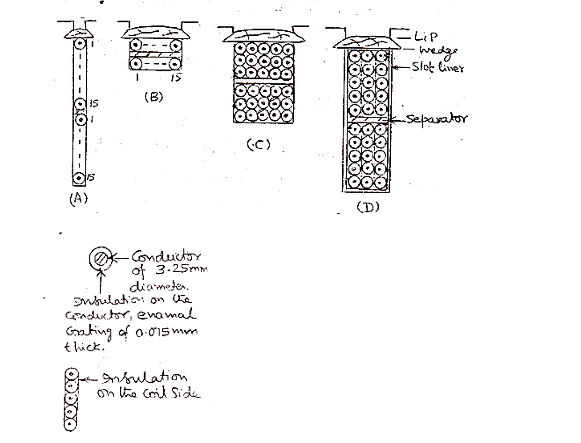
\includegraphics[width=0.9\textwidth]{images/image1}
\end{center}

\begin{itemize}
	\item \textbf{(A)} 15 conductors are arranged one below the other in each layer — the slot becomes too deep and not proportionate.
	\item \textbf{(B)} 15 conductors are arranged side by side in each layer — the slot becomes too wide and not proportionate.
	\item \textbf{(C) \& (D)} Conductors are arranged in a grid pattern — leads to proportionate slot dimensions.
\end{itemize}

If the conductors are arranged as shown in pattern (D), then the slot width is calculated as:

\[
b_s = (\text{diameter of the conductor} + \text{insulation thickness}) \times \text{number of conductors along the slot width}
\]

\[
b_s = (3.25 + 2 \times 0.075) \times 3 = 10.05\, \text{mm}
\]

\vspace{5pt}

\noindent
This arrangement provides a balanced and manufacturable slot design.












\vspace{10pt}

\noindent
\textbf{Slot Width Calculation}

\[
b_s = (\text{diameter of conductor} + 2 \times \text{insulation thickness}) \times \text{number of conductors along width} + \text{insulation over coil sides} + \text{slot liner} + \text{clearance}
\]

\[
b_s = (3.25 + 2 \times 0.075) \times 3 + 1.5 = 11.7\, \text{mm}
\]

\vspace{10pt}

\noindent
\textbf{Slot Depth Calculation}

\[
h = (\text{diameter of conductor} + 2 \times \text{insulation thickness}) \times \text{number of conductors along depth} + (\text{insulation over coil sides} + \text{slot liner} + \text{separator} + \text{clearance}) + \text{wedge thickness} + \text{lip thickness}
\]

\[
h = (3.25 + 2 \times 0.075) \times 10 + 4 + 4 + 2 + 3 + 1 = 44\, \text{mm}
\]

\vspace{10pt}

\noindent
\textbf{Flux Density at One-Third Tooth Height}

The flux density in the tooth at one-third the height from the root is calculated using:

\[
B_{t\,1/3} = \frac{\phi}{b_{t\,1/3} \cdot L_i \cdot \frac{S}{P}}
\]

First, calculate the tooth width at one-third height:

\[
b_{t\,1/3} = \frac{\pi (D - \delta \cdot h/3)}{S} - b_s
\]

\[
b_{t\,1/3} = \frac{\pi (54 - \delta \cdot 44 / 3)}{60} - 1.17 = 1.35\, \text{cm}
\]

Next, compute the net iron length:

\[
L_i = K_i (L - n_b \cdot b_0) = 0.9 (24.5 - 2 \cdot 1) = 20.7\, \text{cm}
\]

Now, calculate the flux density:

\[
B_{t\,1/3} = \frac{0.038}{0.0135 \cdot 0.207 \cdot \frac{60}{6}} = 1.367\, \text{T}
\]

This value is slightly higher than the average due to flux concentration under the pole arc.

\vspace{10pt}

\noindent
\textbf{Maximum Flux Density in the Enclosure}

Assuming the per-unit enclosure flux $\psi = 0.7$, the maximum flux density is given by:

\[
(B_{t\,1/3})_{max} = \frac{1.36}{0.7} = 1.94\, \text{T}
\]

Since $1.94\, \text{T} < 2.1\, \text{T}$, the design is within the acceptable limit.







\end{document}
